 %\documentclass[wcp,gray]{jmlr} % test grayscale version
 %\documentclass[wcp]{jmlr}% former name JMLR W\&CP
\documentclass[pmlr]{jmlr}% new name PMLR (Proceedings of Machine Learning)

 % The following packages will be automatically loaded:
 % amsmath, amssymb, natbib, graphicx, url, algorithm2e

 %\usepackage{rotating}% for sideways figures and tables
\usepackage{longtable}% for long tables

 % The booktabs package is used by this sample document
 % (it provides \toprule, \midrule and \bottomrule).
 % Remove the next line if you don't require it.
\usepackage{booktabs}
 % The siunitx package is used by this sample document
 % to align numbers in a column by their decimal point.
 % Remove the next line if you don't require it.
\usepackage[load-configurations=version-1]{siunitx} % newer version
 %\usepackage{siunitx}

% Package to make table with multi rows and columns
\usepackage{multirow}
 
 % to do
\usepackage{xcolor}
\newcommand\todo[1]{\textcolor{red}{#1}}

 % change the arguments, as appropriate, in the following:
\jmlrvolume{1}
\jmlryear{2019}
\jmlrworkshop{}


% start article
% \titlebreak
% \footnote{}
% \textsf

\title[Conformal Prediction for Students' Grades]{Conformal Prediction for Students' Grades in a Course Recommender System}	%\titletag{\thanks{XXX}} % leave empty?

 % Use \Name{Author Name} to specify the name.
 % If the surname contains spaces, enclose the surname
 % in braces, e.g. \Name{John {Smith Jones}} similarly
 % if the name has a "von" part, e.g \Name{Jane {de Winter}}.
 % If the first letter in the forenames is a diacritic
 % enclose the diacritic in braces, e.g. \Name{{\'E}louise Smith}

 % Authors with different addresses:
  \author{\Name{Rapha\"{e}l Morsomme} \Email{raphael.morsomme@maastrichtuniversity.nl}\\ % Morsomme\nametag{\thanks{with a note}} % leave this slot empty?
   \addr Zwingelput 4, 6211 KH Maastricht, the Netherlands	
   \AND
   \Name{Evgueni Smirnov} \Email{smirnov@maastrichtuniversity.nl}\\
   \addr Bouillonstraat 10, 6211 LH Maastricht, the Netherlands}

 % Three or more authors with the same address:
 % \author{\Name{Author Name1} \Email{an1@sample.com}\\
 %  \Name{Author Name2} \Email{an2@sample.com}\\
 %  \Name{Author Name3} \Email{an3@sample.com}\\
 %  \addr Address}

 % Authors with different addresses:
 % \author{\Name{Author Name1} \Email{abc@sample.com}\\
 % \addr Address 1
 % \AND
 % \Name{Author Name2} \Email{xyz@sample.com}\\
 % \addr Address 2
 %}

% leave editor's section empty?
%\editor{Editor's name}
% \editors{List of editors' names}

\begin{document}

\maketitle

\begin{abstract}
Course selection can be challenging for student of Liberal Arts programs. In particular, due to the highly personalized curricula of liberal arts students, it is often difficult to assess whether or not a particular course is too advanced given their academic background. To assist students of the liberal arts program of the University College Maastricht, \citet{Morsomme.2019} developed a course recommender system that suggests courses whose content matches the student's academic interests, and issues warnings for courses that it deems too advanced.

To issue warnings, the system produces point predictions for the grades that a student will receive in the courses that she/he is considering for the following term. Point predictions are estimated with regression models specific to each course which take into account the academic performance of the student along with the knowledge that she/he has acquired in previous courses. A warning is issued if the predicted grade is a fail.

In this paper, we complement the system's point predictions for grades with prediction intervals constructed using the conformal prediction framework \citep{Vovk.2005}. We use the Inductive Confidence Machine (ICM) \citep{Papadopoulos.2002} with standardized nonconformity scores to construct prediction intervals that are tailored to each student. We find that the prediction intervals constructed with the ICM are valid and that their widths are related to the accuracy of the underlying regression model.
\end{abstract}

\begin{keywords} Conformal Prediction, Recommender System, Course Grade Prediction, Lasso, Education \end{keywords}

% \todo{Rapha\"{e}l: make all figures black and white}

% \todo{Rapha\"{e}l: make sure that all figures have the same font size as the main text}

% \todo{Rapha\"{e}l: use notation Z_k = (x_k, y_k) to simplify description of conformal prediction}

\section{Introduction}
\label{sec:intro}

Liberal Arts programs are often characterized by their open curriculum which allows student to tailor their own study program to their academic objectives \citep{Surpatean.2012, Morsomme.2019}. These highly personalized curricula make it difficult for students, academic advisors and course coordinators to assess whether the courses that a student considers taking the following term are too advanced given her/his current academic background or whether she/he has acquired the necessary skills, perhaps through an unusual combination of courses. To alleviate this problem, \citet{Morsomme.2019} developed the Liberal Arts Recommender System (LARS) which suggests to students courses whose content matches their academic interests. In addition, LARS helps student identify courses that are too advanced for them. To accomplish that, the system issues \textit{point predictions} for future grade based on the past academic performance of the student and the skills she/he has acquired in previous courses. A warning is issued when the predicted grade is a fail.

In this paper, we present an application of conformal prediction \citep{Vovk.2005} to complement the current point estimates for future grades of LARS with prediction intervals. For students, the advantage of prediction intervals over point predictions is clear: their information position is improved, thereby enabling them to make better-informed course selection. To avoid the computational costs of transductive conformal prediction, we opt for the lighter Inductive Confidence Machine (ICM) \citep{Papadopoulos.2002}. Furthermore, in order to provide prediction intervals that are tailored to each student, we use a normalized nonconformity measure \citep{Papadopoulos.2011}.

\sectionref{sec:related} presents previous research on grade prediction.
\sectionref{sec:data} introduces the data and \sectionref{sec:crs} briefly describes the existing LARS.
\sectionref{sec:prediction} presents the conformal prediction framework in which we construct the prediction intervals.
\sectionref{sec:experiment} presents the setting and results of the experiment
and \sectionref{sec:conclusion} concludes.

\section{Related Work}
\label{sec:related}

The task of predicting students' course grades prediction has recently received a lot of attention \citep{Polyzou.2016, Houbraken.2017}. The approaches to this problem are regression approaches, classification approaches, and collaborative-filtering approaches. The first two approaches employ general information (secondary education, age, sex etc.), past performance, temporal elements, and contextual information of the students \citep{Bydzovska.2016}. They train a regression/classification model on historical data which is latter used for predicting students' course grades. The collaborative-filtering approaches require only past course grades for future prediction in contrast with the previous two approaches \citep{Sweeney.2015, Houbraken.2017}. They are divided into nearest-neighbor approaches \citep{Bydzovska.2015} and matrix-factorization approaches \citep{Polyzou.2016}. The nearest-neighbor approaches first identify neighbors of a student in terms of study performance and then predict the course grades for this student by aggregating the course grades of the neighbors. The matrix factorization approaches first decompose the student-course data into student and course matrices and then predict student course grades using the product of these matrices.

Although the progress in  student course grade prediction is significant, no research was performed on the problem of estimating the confidence in this type of prediction. As it is stated above we propose to employ conformal prediction for this problem. Our choice is justified by the fact that other approaches for reliable prediction such as version spaces \citep{Smirnov.2004}, meta approaches \citep{Smirnov.2006, Smirnov.2006b}, ROC-isometric approaches \citep{Vanderlooy.2006} are 
inapplicable for regression tasks.

\section{Data for LARS}
\label{sec:data}

\citet{Morsomme.2019} employed two sets of data to develop LARS: student data and course data.

The student data consisted of anonymized course enrollment information. It included the transcripts of the 2,526 students of the liberal arts program between 2008 and 2019 with a total of 79,245 course enrollments. Course enrollments with a missing grade, which indicates that the student either dropped the course or fail the attendance requirement, were removed. \tableref{tab:student-data} presents an example of the student data. Each row contains an anonymized student ID, a course ID, a year and semester, and the obtained grade.

The course data consisted of a corpus of the 490 course descriptions present in the 2018-2019 course catalogues of five departments of Maastricht University: European Studies, University College Maastricht, University College Venlo, Psychology and Science Program. These catalogues contain a one-page description of each course on offer. \tableref{tab:course-data} presents a sample of this textual data for the course \textit{HUM3034 World History} in the tidy format with one row per document-term \citep{Wickham.2014}. The data was processed following common procedures \citep{Meyer.2008}: individual terms were tokenized, stemmed with the Hunspell dictionary and common stop words were removed, as well as numbers between 1 and 1,000 and terms occurring less than 3 times in the corpus.

\begin{table}[hbtp]
	\floatconts
	{tab:student-data}
	{\caption{Example of student data}}	
	{\begin{tabular}{ccccc}
		\toprule
		\bfseries Student ID &\bfseries Course ID &\bfseries Academic Year &\bfseries Period &\bfseries Grade\\
		\midrule
		44940 & CAP3000 & 2009-2010 & 4 & 8.8\\
		37490 & SSC2037 & 2009-2010 & 4 & 8.4\\
		71216 & HUM1003 & 2010-2011 & 4 & 6.8\\
		44212 & SSC2049 & 2010-2011 & 2 & 8.4\\
		85930 & SSC2043 & 2011-2012 & 1 & 4.3\\
		\addlinespace
		14492 & COR1004 & 2012-2013 & 2 & 8.5\\
		34750 & HUM2049 & 2013-2014 & 5 & 6.0\\
		32316 & SSC1001 & 2013-2014 & 1 & 8.5\\
		22092 & SCI1009 & 2014-2015 & 1 & 6.4\\
		19512 & COR1004 & 2016-2017 & 5 & 7.0\\
		\bottomrule
	\end{tabular}}	
\end{table}

\begin{table}[hbtp]
	\floatconts
	{tab:course-data}
	{\caption{Example of course data for the course HUM3034 World History}}	
	{\begin{tabular}{cccc}
			\toprule
			\bfseries Course ID &\bfseries Course Title &\bfseries Department &\bfseries Term\\
			\midrule
			HUM3034 & World History & UCM & understand\\
			HUM3034 & World History & UCM & major\\
			HUM3034 & World History & UCM & issue\\
			HUM3034 & World History & UCM & episode\\
			HUM3034 & World History & UCM & shape\\
			\addlinespace
			HUM3034 & World History & UCM & history\\
			HUM3034 & World History & UCM & mankind\\
			HUM3034 & World History & UCM & focus\\
			HUM3034 & World History & UCM & theme\\
			HUM3034 & World History & UCM & topic\\
			\bottomrule
	\end{tabular}}	
\end{table}

\section{LARS}
\label{sec:crs}
\subsection{Overview}
\label{sec:overview}

LARS is composed of two pillars: course suggestions and warning issuance (see \figureref{fig:flowchart}). 

In pillar 1, a topic model of the courses is fitted to the course data using the Latent Dirichlet Allocation model \citep{Blei.2003}. A topic model represents a topic as a mixture of words and a document as a mixture of topics. The key words selected by the student are then mapped to the vocabulary of the topic model to represent her/his academic interests. Finally, the system matches the student's academic interests to the content of the courses as represented by the topic model to identify courses of interest to the student.

In pillar 2 for warning issuance, a model of each student is first created which contains information about the academic performance of the student (derived from the student data) and the expertise in specific topics (derived from the topic model) that she/he has acquired in previous courses. A regression model for point prediction of the grades that takes the student model as input is then fitted for each course. LARS uses these models to predict the grade that the student will obtain in the courses that she/he is considering for the following term and issues a warning when the predicted grade is a fail.

\begin{figure}[htbp]
	\floatconts
	{fig:flowchart}
	{\caption{Original LARS (black) and our contribution (red)}}
	{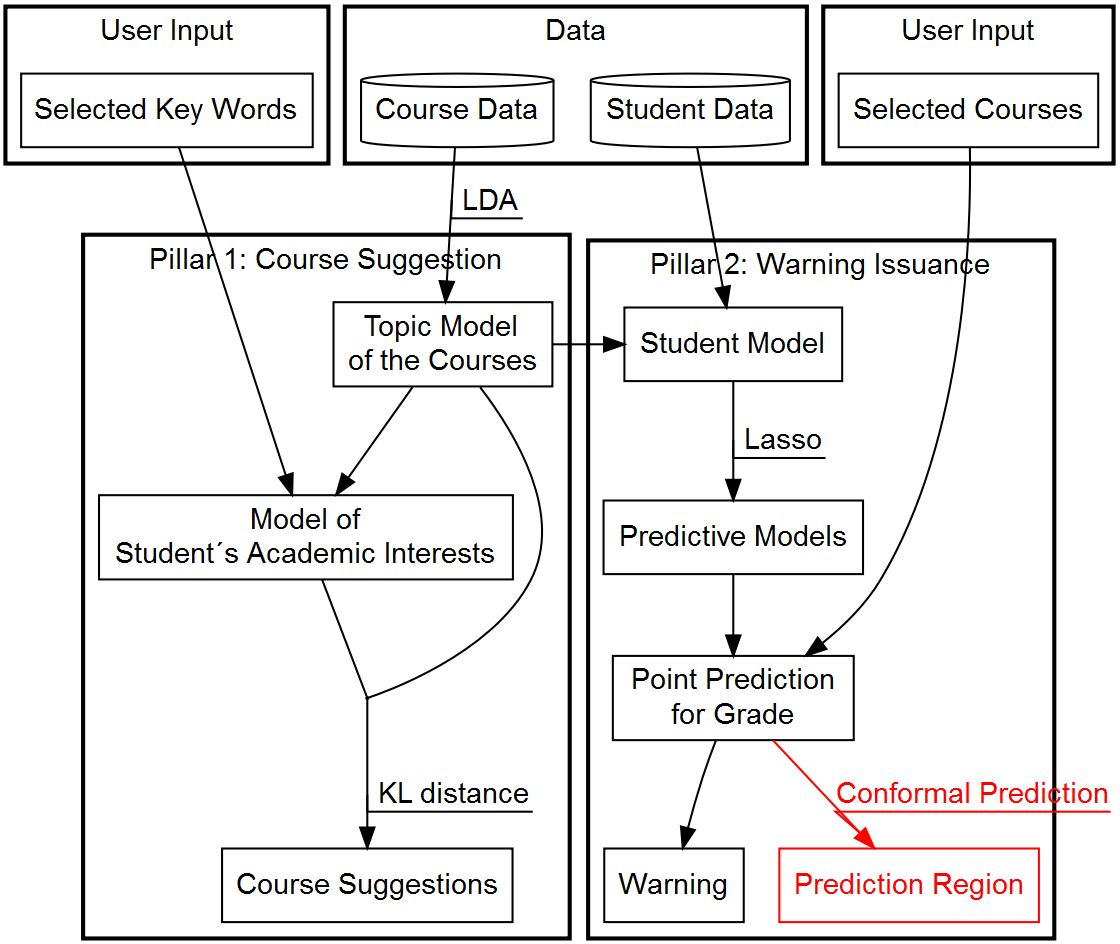
\includegraphics[width=0.66\linewidth]{figures/flowchart}}
\end{figure}

\subsection{Pillar 1: Course Suggestion}

\subsubsection{Topic Model of the Courses}
\label{sec:tm}

\citet{Morsomme.2019} fitted a topic model to the course data using the Latent Dirichlet Allocation generative model \citep{Blei.2003} and the Gibbs sampling algorithm \citep{Phan.2008}. The LDA conceptualizes topics as a probability distribution over the vocabulary of the corpus, and document as a set of words, each drawn from a probability distribution over topics specific to that document. The term \textit{Dirichlet} comes from the fact that the word distribution $\beta_{t}$ of topic $t$ is generated from a Dirichlet distribution $\beta_{t} \sim Dirichlet(\delta)$ and the topic distribution $\theta_{d}$ for document $d$ is generated from a Dirichlet distribution $\theta_{d} \sim Dirichlet(\alpha)$ where $\delta$ and $\alpha$ act as hyper-parameters determining how concentrated the distributions of words in topics and the distributions of topics in documents are.

The authors of LARS followed \citet{Phan.2008} who use a Gibbs sampler to learn the distributions $\beta$ and $\theta$ of each topic and document, and \citet{Griffiths.2004} who select the number of topics yielding the best model with respect to the log-likelihood. The selected topic model contains 65 topics (see \figureref{fig:ll}) and consists of a term distribution for each topic indicating the importance of each term of the corpus in the topic and a topic distribution for each course indicating the importance of each topic in the course. \figureref{fig:gamma} shows the main topics of the core course \textit{COR1004 Political Philosophy} and \figureref{fig:beta} presents the terms that characterize topic 4 and topic 19, the main two topics of the course. We can see that the topics are easy to interpret and that the content of the course, that is, its topic distribution, corresponds to what we would expect from a course on political philosophy.

\begin{figure}[htbp]
	\floatconts
	{fig:ll}
	{\caption{Maximum likelihood model selection: the model with 65 topics is selected.}}
	{\includegraphics[width=0.5\linewidth]{figures/model-selection}}
\end{figure}

\begin{figure}[htbp]
	\floatconts
	{fig:gamma}
	{\caption{Topic distribution in the course COR1004 Political Philosophy.}}
	{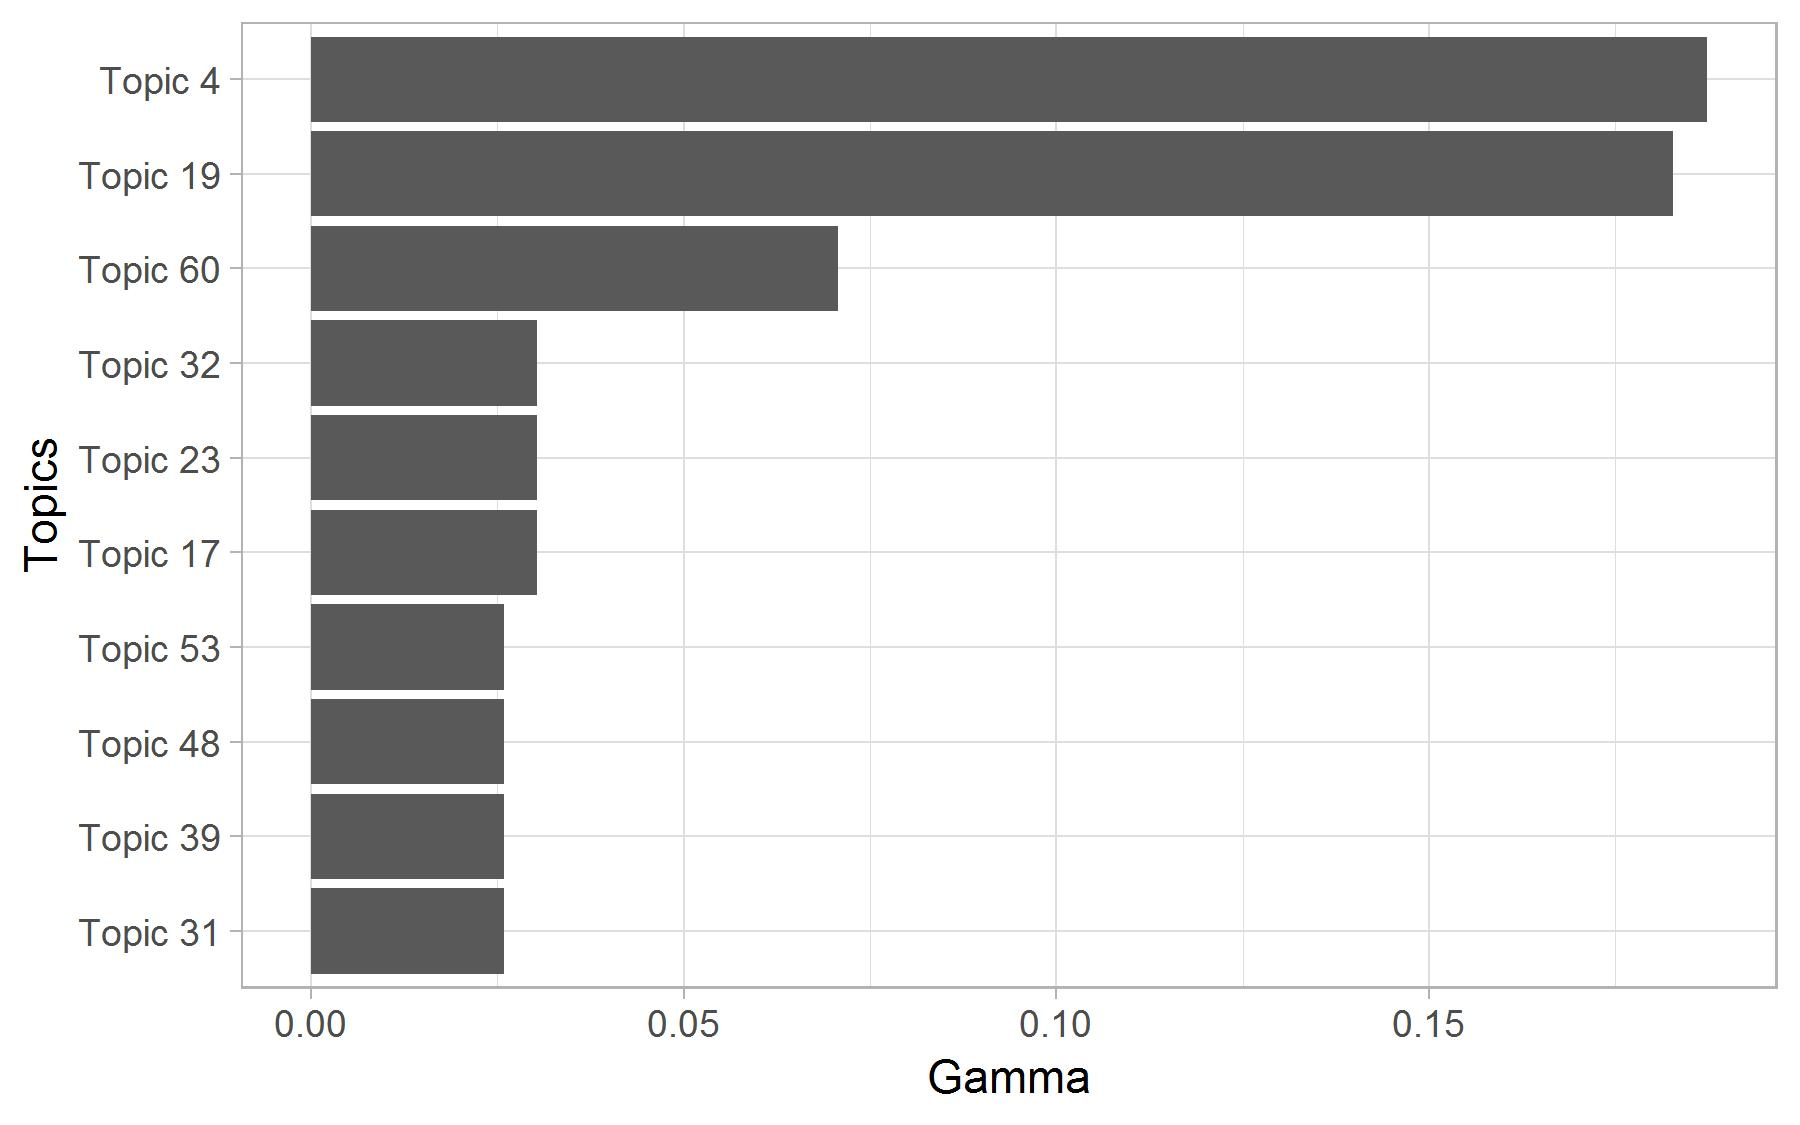
\includegraphics[width=0.5\linewidth]{figures/gamma-COR1004}}
\end{figure}

\begin{figure}[htbp]
	\floatconts
	{fig:beta}
	{\caption{Word distribution in the main two topics of COR1004 Political Philosophy. Topic 4 corresponds to international politics and Topic 19 to philosophy.}}
	{\includegraphics[width=0.75\linewidth]{figures/beta}}
\end{figure}

\subsubsection{Model of a Student's Academic Interests}

\citet{Morsomme.2019} employed the topic model to estimate the academic interests of a student from the key words that she/he enters into the system. The student's academic interest $AI_t$ in topic $t$ simply corresponds to the sum of the selected key words' importance in topic $t$ as determined by the topic model, that is,
$$ AI_t = \sum_{i \in I^*} \beta_{t,i}, \;\;\;  \mbox{for} \;\;\;  t=1, \cdots, n,$$
where $I^*$ is the set of key words selected by the student, $\beta_{t,i}$ corresponds to the importance of term $i$ in topic $t$ and $n$ is the number of topics present in the model (in this case $n=65$). The vector $AI = (AI_1, \cdots, AI_{n})^T$ therefore represents the academic interests of the student.

\subsubsection{Course Matching and Suggestion}

LARS uses the Kullback-Leibler (KL) divergence \citep{Kullback.1951} to identify the courses whose content best matche the academic interests of the student.
Letting $P$ and $Q$ be two discrete probability distribution defined on the same probability space, the KL divergence between $P$ and $Q$ is defined as

$$ D_{\mathrm{KL}} \left( P || Q \right) =  - \sum_{x \in X} P(x) \log\left(\dfrac{Q(x)}{P(x)}\right)$$

\noindent and measures how different the probability distribution $P$ is from the reference probability distribution $Q$.
LARS suggests to the students the $n$ courses whose topic distribution $\theta$ has the smallest KL divergence to her/his normalized academic interests $AI^* = \dfrac{AI}{\lvert AI \rvert}$.

\subsection{Pillar 2: Warning Issuance}
\subsubsection{Student Model}
\label{sec:sm}
The student model consists of two elements: academic performance and topic-specific expertise. Academic performance corresponds to the student's general GPA (grade point average) as well as her/his GPA in humanities, natural sciences, social sciences, skills and projects. These are derived from the students' transcripts in a straightforward way. Topic-specific expertise corresponds to the amount of knowledge that the student has acquired  in previous courses in each of the topics present in the topic model. \citet{Morsomme.2019}  posited that, when students take a course, they acquire knowledge about its content and that the amount of knowledge that they acquire is proportional to the obtained grade; that is, they assume that students who obtain 10/10 in a course acquire all the knowledge related to its content while those who obtain 5/10 only acquire half of it. The content of a course is determined by its topic distribution in the topic model and the grades are retrieved from the student's transcript. Furthermore, they assume that the knowledge acquired in different courses simply accumulates. Hence, if a student has taken $n$ courses and $g_{i}$ corresponds to her/his grade in course $i$, for $i = 1, \cdots, n$, then her/his expertise $exp_t$ in topic $t$ corresponds to

\begin{equation}
\label{eq:expertise}
exp_t = \sum_{i= 1}^{n} g_i \theta_{i,t}
\end{equation}

\noindent where $\theta_{i,t}$ corresponds to the importance of topic $t$ in course $i$ as determined by the topic model. \tableref{tab:toy} and \figureref{fig:toy-expertise} present a toy example of the contribution of three individual courses toward a student's expertise in five topics. \tableref{tab:toy-gamma} and \tableref{tab:toy-grade} respectively show the topic distribution in each course as estimated by some topic model and the grades obtained by the student which are retrieved from her/his transcript. \tableref{tab:toy-contribution} uses \equationref{eq:expertise} to estimate the contribution of each course toward the student's topic expertise. \figureref{fig:toy-expertise} offers a graphical illustration of \tableref{tab:toy-contribution}.

\begin{table}[htbp]
	\floatconts
	{tab:toy}
	{\caption{Toy example of the contribution of individual courses toward a student's topic expertise.}}
	{%
		\subtable[Topic distribution $\theta$]{%
			\label{tab:toy-gamma}%
			\begin{tabular}{cccccc}
				\toprule
				\bfseries Course & \bfseries Topic 1 & \bfseries Topic 2 & \bfseries Topic 3 & \bfseries Topic 4 & \bfseries Topic 5\\
				\midrule
				Course 1 & 0.0 & 0.7 & 0.2 & 0.1 & 0.0\\
				Course 2 & 0.2 & 0.2 & 0.2 & 0.2 & 0.2\\
				Course 3 & 0.0 & 0.4 & 0.2 & 0.1 & 0.2\\
				\bottomrule
			\end{tabular}
		}\qquad
		\subtable[Transcript]{%
			\label{tab:toy-grade}%
			\begin{tabular}{cc}
				\toprule
				\bfseries Course & \bfseries Grade\\
				\midrule
				Course 1 & 6/10\\
				Course 2 & 9/10\\
				Course 3 & 2/10\\
				\bottomrule
			\end{tabular}
		}\qquad
			\subtable[Course contribution toward a student's topic expertise]{%
			\label{tab:toy-contribution}%
			\begin{tabular}{cccccc}
				\toprule
				\bfseries Course & \bfseries Topic 1 & \bfseries Topic 2 & \bfseries Topic 3 & \bfseries Topic 4 & \bfseries Topic 5\\
				\midrule
				Course 1 & 0.00 & 0.42 & 0.12 & 0.06 & 0.00\\
				Course 2 & 0.18 & 0.18 & 0.18 & 0.18 & 0.18\\
				Course 3 & 0.00 & 0.08 & 0.04 & 0.02 & 0.04\\
				\midrule
				\bfseries Total & 0.18 & 0.68 & 0.34 & 0.26 & 0.22\\
				\bottomrule
			\end{tabular}
		}
	}
\end{table}

\begin{figure}[htbp]
	\floatconts
	{fig:toy-expertise}
	{\caption{Toy example of the contribution of individual courses toward a student's topic expertise.}}
	{\includegraphics[width=0.5\linewidth]{figures/toy-expertise}}
\end{figure}

\subsubsection{Point Prediction for Grade and Warning Issuance}

To issue warnings, LARS produces point estimates for future grades. To accomplish this, it uses regression models.  LARS separately fits a sparse linear regression model for grade prediction to each of the 132 courses currently offered at the University College Maastricht with at least 20 student enrollments since 2008. The input to the models consists of the 71 variables stored in the student model: 6 GPAs (1 general and 5 discipline-specific) and the level of expertise in the 65 topics of the topic model. The regression models output a point estimate for the grade. Note that each model is trained only on the data of the students enrolled in the associated course. Since the number of predictors is relatively large, the models are regularized with the Lasso penalty \citep{Tibshirani.1996} and the value of the Lasso tuning parameter $\lambda$ is chosen via cross-validation (CV). \figureref{fig:cv-mae} shows the distribution of the CV mean absolute error (mae) for the 132 prediction models. The model for the course \textit{PRO2004 Academic Debate} has the smallest prediction error (0.38 grade point) and the model for \textit{SCI3006 Mathematical Modelling} the largest (1.80 grade point). The mean CV mae weighted by the number of students enrolled in the course is 0.78, the median is 0.78 and the standard deviation is 0.28.

% use cross-validation to find the value of the Lasso tuning parameter $lambda$ that minimizes the CV mean absolute error (mae), a more robust loss function than the squared absolute error \citep{Hastie.2009}

\begin{figure}[htbp]
	\floatconts
	{fig:cv-mae}
	{\caption{Distribution of cross-validation error}}
	{\includegraphics[width=0.5\linewidth]{figures/cv-mae}}
\end{figure}

In practice, the student selects the courses that she/he is considering for the following term and the system uses the regression models of these courses to provide point predictions for the future grades. A warning is issued when a predicted grade is a fail.

We desire the following three requirements for pillar 2 Warning Issuance of LARS: accuracy, sparsity and transparency of the regression models for grade prediction. First, the grade predictions must be accurate so that students base their course selection on sound information. Second, we want the regression models to be sparse so that we can identify which topics are important to master in order to perform well in a given course. Such information would be extremely useful to course coordinators and curriculum managers alike. Third, in order to be transparent, grade predictions must be accompanied by an indication of their own accuracy. The first two requirements are fulfilled by the Lasso model \citep{Tibshirani.1996}, but the third requirement is not satisfied by LARS's current \textit{point predictions} for future grades. To fulfill the requirement for transparency, we propose to complement the existing point predictions of the system with \textit{prediction intervals}. In the following section, we use the conformal prediction framework to build prediction intervals for future grades that are tailored to each student.

\section{Regression with Prediction Interval}
\label{sec:prediction}

Let $X$ be a space given by $n$ input variables $X_j$ ($j \in \{1, 2, \ldots, n\}$) and $Y$ be an output real-value variable. Any $i$-th instance in the labeled space  $(X \times Y)$ is given as a tuple $(x_i, y_i)$ where $x_i$ belongs to $X$, $x_{ij}$ is the value for the input variable $X_j$ for the instance $x_i$, and $y_i$ is the value for the output variable $Y$. We assume the existence of an unknown  probability distribution $P$ over $X \times Y$.  A data set $D$ is a multi-set of $m$ instances $(x_i, y_{i}) \in (X \times Y)$ drawn from the probability distribution $P$ under the randomness assumption.  Given an unlabeled test  instance $x_{m+1} \in X$,  the regression  task  is to find an estimate $\hat{y}_{m+1} \in \mathbb{R}$ of the value of the variable $Y$ for the instance $x_{m+1}$ according to the probability distribution $P$. A  prediction interval $\Gamma^\epsilon$ for the test instance $x_{m+1}$ is defined as the set $\{ y \in \mathbb{R}| p(y) > \epsilon\}$ that contains the true value of the output variable $Y$ for $x_{m+1}$ with probability of at least $1- \epsilon$, where $\epsilon$ is a given significance level.

\subsection{Underlying Algorithm: Lasso Regression}
\label{sec:lasso}

Lasso is a parametric method for regression that allows regularization and variable selection \citep{Tibshirani.1996}. The method estimates the coefficients of the final regression model by minimizing:

\[ \sum_{i = 1}^{m} ( y_i - \beta_0 - \sum_{j = 1}^{n} \beta_j x_{ij})^2 + \lambda \sum_{j = 1}^{n}\lvert\beta_j\rvert, \]

\noindent i.e., by minimizing the  residual sum of the squares $\sum_{i = 1}^{m} ( y_i - \beta_0 - \sum_{j = 1}^{n} \beta_j x_{ij})^2$ and the Lasso penalty $\lambda \sum_{j = 1}^{n}\lvert\beta_j\rvert$.

The Lasso method shrinks the coefficient estimates $\hat{\beta}_j$ toward 0. This reduces the variance of the model and thereby helps preserve its prediction accuracy. Furthermore, in contrast to the ridge regression penalty, the absolute-value constraint of Lasso encourages some of the coefficient estimates to be exactly zero and hence the regression model to be sparse. This facilitates the interpretation of the obtained models.

\subsection{Conformal Prediction and the Inductive Conformal Machine}
\label{sec:cp}

The conformal prediction framework was proposed by \citet{Vovk.2005}. It allows the construction of  prediction intervals for regression tasks in the presence of finite data sets generated under the exchangeability assumption (which is weaker than the randomness assumption). In general, conformal predictors are conservatively valid; that is, the probability that any prediction interval $\Gamma^\epsilon$ does not contain the true value is not greater than $1 - \epsilon$.

The conformal prediction framework assumes a nonconformity function $A$. The function outputs a nonconformity score $\alpha_k \in \mathbb{R}^+ \cup \{+\infty\}$ for any instance $(x_{k},y_{k})$ that indicates how unusual that instance is for the data set $D \cup \{(x_{m+1},y_{m+1})\}$. For the regression setting, a popular choice for the nonconformity score $\alpha_k$ of an instance $(x_{k},y_{k})$ is the residual $|y_k - \hat{y}_k|$, where $\hat{y}_k$ is the estimation for the variable $Y$ for the instance $x_k$ provided by some underlying regression model based on the data set $D \cup \{(x_{m+1}, y_{m+1})\}$ \citep{Papadopoulos.2002, Papadopoulos.2015}. In this paper we employ a normalized nonconformity score for the instance  $(x_{k},y_{k})$ corresponding to

\begin{equation}
\label{eq:norm}
\alpha_k = \frac{\lvert y_k - \hat{y}_k\rvert}{\exp(\mu_k)}
\end{equation}

\noindent where $\mu_k$ is the prediction of the value $\ln \lvert y_k - \hat{y}_k \rvert$ from a second regression model \citep{Papadopoulos.2011}. The intuition behind equation (\equationref{eq:norm}) is that by taking into account the expected accuracy of the underlying regression model, we do not inflate the nonconformity score of instances that are intrinsically difficult to predict.

Once the nonconformity scores have been computed for all the instances in the data set  $D \cup \{(x_{m+1},y_{m+1})\}$, the $p$-value $p_{m+1}$ for the output value  $y_{m+1}$ for the instance $x_{m+1}$ corresponds to the proportion of instances in $D \cup \{(x_{m+1},y_{m+1})\}$ whose nonconformity score is greater than or equal to that of the instance $(x_{m+1},y_{m+1})$; i.e.

\begin{equation}
\label{eq:p}
p_{m+1} = \frac{\#\{i= 1,...,m|\alpha_i \geq \alpha_{m+1}\} }{m+1}.
\end{equation}

Depending on the validation procedure for estimating the nonconformity scores, there exist two approaches to generate valid conformal predictors. First, the \textit{transductive conformal predictors} (TCP) proposed by \citet{Saunders.1999} uses \textit{leave-one-out} cross-validation and is computationally expensive. To reduce the computational burden, the \textit{inductive conformal machine} (ICM) was proposed by \citet{Papadopoulos.2002}. It employs the hold-out method: the data $D$ is partitioned into a proper training set $D_t$ of size $p$ and a proper calibration set $D_c$ of size $q$ ($D = D_t \cup D_c$ and $m = p + q$). The proper training set $D_t$ is used to learn the nonconformity function $A$. The function is learned by training two regression models: the \textit{target} model and the \textit{error} model. The target model estimates the values $y_k$ which we need to estimate the residuals $\lvert y_k - \hat{y}_k\rvert$. The error model estimates the accuracy $\mu_k = \ln \lvert y_k - \hat{y_k} \rvert$ of the target model (see \equationref{eq:norm}). The use of the natural logarithm and exponent prevents the estimated residuals -- and hence the nonconformity scores -- to be negative. The regression models are then applied to the instances of the calibration set $D_c$ to compute their nonconformity scores $\alpha$.

Once the nonconformity scores have been computed for the instances of the calibration set $D_c$, the $p$-value $p_{m+1}$ for the output value $y_{m+1}$ for the instance $x_{m+1}$ corresponds to the proportion of instances in $D_c$ whose nonconformity score is greater than or equal to that of the instance $(x_{m+1},y_{m+1})$; i.e.

\begin{equation}
\label{eq:e3}
p_{m+1} = \frac{\#\{i= p+1,...,m|\alpha_i \geq \alpha_{m+1}\} }{m - p +1}. 
\end{equation}

The nonconformity scores of the calibration instances can be used for constructing a prediction interval for the test instance $x_{m+1}$. To accomplish this, the nonconformity scores are sorted in increasing order of magnitude: $ \alpha_{(1)}, \alpha_{(2)}, \ldots, \alpha_{(q)}$. The prediction interval for the test instance $x_{m+1}$ is constructed as:

\begin{equation}
\label{eq:e4}
(\hat{y}_{m+1} - \alpha_{(s)} , \hat{y}_{m+1} + \alpha_{(s)})
\end{equation}

\noindent where  $\hat{y}_{m+1} $  is the value of the variable $Y$ for the instance $x_{m+1}$ estimated by the target regression model trained on the proper training set $D_t$, $s = \lfloor \epsilon (|q|+1) \rfloor$, and $\epsilon$ is a given significance level \citep{Papadopoulos.2011}. We note that the construction of prediction intervals is model-independent: prediction intervals can be constructed for any type of regression model.

\section{Experiments}
\label{sec:experiment}

\subsection{Settings}

We separately build a regression model for grade prediction for each of the 132 courses currently offered at the University College Maastricht with more than 20 student enrollments since 2008. To build these models, we use an ICM with normalized nonconformity scores. For each model, the data consists of the  models of the students enrolled in the associated course. A student model data consists of the 6 GPAs (1 general and 5 discipline-specific) of a student along with her/his level of expertise in the 65 topics of the topic model at the beginning of the course (see \sectionref{sec:sm}).

We choose the target model to be a lasso-penalized linear regression model because it fulfills the requirements for accuracy and sparsity. We also choose the error model to be a lasso regression. We first fit the target model on the proper training set (66\% of the data) to estimate grades. We then fit the error model on the proper training set too to estimate the accuracy of the target model. Note that both models learn the lasso tuning parameter $\lambda$ with an internal 10-fold cross-validation on the proper training set. Finally, using \equationref{eq:e3,eq:e4}, we construct prediction intervals for each test instance  at several significance levels and evaluate their validity and tightness. We report the final results for an external 10-fold cross-validation.

\subsection{Results}

We present the results for a selection of six courses which cover a wide range of sample size and of cross-validation mean absolute error (CV mae) for the target model (see \tableref{tab:conformal-course}). \textit{SSC3044 Culture, Politics and Society in Contemporary Asia} and \textit{SSC3038 Contemporary Sociological Theory} have a small CV mae ($\le0.4$ point grade), while \textit{SCI2010 Introduction to Game Theory} and \textit{SCI2018 Calculus} have a large CV mae ($\ge1.4$). Since they are mandatory, the courses \textit{COR1004 Political Philosophy} and \textit{COR1002 Philosophy of Science} have a large sample size ($n\ge1900$), while \textit{SSC3044 Culture, Politics and Society in Contemporary Asia} and \textit{SCI2018 Calculus} have a much fewer observations ($n\le200$).

\begin{table}[hbtp]
	\floatconts
	{tab:conformal-course}
	{\caption{Selected courses for conformal prediction}}	
	{\begin{tabular}{ccccc}
			\toprule
			\bfseries Course &\bfseries Sample Size &\bfseries CV mae \\
			\midrule
			SSC3044 & 136  & 0.38\\
			SSC3038 & 272  & 0.40\\
			COR1004 & 1998 & 0.67\\
			COR1002 & 2067 & 1.00\\
			SCI2010 & 417  & 1.41\\
			SCI2018 & 198  & 1.62\\
			\bottomrule
	\end{tabular}}	
\end{table}

\tableref{tab:conformal-summary} and \figureref{fig:conformal-error} present the error rate of the prediction intervals constructed with the ICM at different significance levels for each course, that is, the proportion of intervals that do not contain the true grade of the student. We see that the prediction intervals are conservatively valid; that is, given a significance level, the probability that a prediction interval does not contain the true value is not greater than the significance level.

\figureref{fig:conformal-width} shows the distribution of prediction interval width across different significance levels for each course. The dots correspond to the median of the distributions and the bars to the 10th and 90th percentiles. The width $1$ is highlighted for reference. We observe that the width varies across courses. The ICM produces relatively narrow intervals for the course COR1004, SSC3038 and SSC3044 which tend to be less than 1 unit wide for most levels of significance. But for SCI2010 and SCI2018, the interval become wide very quickly: they are wider than 1 unit at significance levels as large as $0.5$. In fact, the prediction interval width seems to be associated with the CV mae: courses with a small CV mae, such as SSC3044, SSC3038 and COR1004, have relatively tight intervals while those with a large CV mae, such as SCI2010 and SCI2018, have wide intervals.

\begin{table}[hbtp]
	\floatconts
	{tab:conformal-summary}
	{\caption{Prediction interval tightness and empirical validity of the ICM.}}	
	{\begin{tabular}{cccccccccc}
			\toprule
			\multirow{2}{*}{\bfseries Course} & \multicolumn{3}{c}{\bfseries Median Width} & \multicolumn{3}{c}{\bfseries Error Rate}\\
			& \bfseries 0.05 & \bfseries 0.1 & \bfseries 0.2 & \bfseries 0.05 & \bfseries 0.1 & \bfseries 0.2\\
			\midrule
			COR1002 & 2.39 & 1.93 & 1.46 & 0.05 & 0.10 & 0.20\\
			COR1004 & 1.63 & 1.29 & 1.01 & 0.05 & 0.10 & 0.19\\
			SCI2010 & 3.69 & 2.86 & 2.18 & 0.05 & 0.12 & 0.22\\
			SCI2018 & 4.68 & 4.02 & 3.05 & 0.04 & 0.08 & 0.17\\
			SSC3038 & \bfseries 0.91 & \bfseries 0.72 & \bfseries 0.50 & 0.07 & 0.14 & 0.23\\
			SSC3044 & 1.02 & 0.84 & 0.63 & 0.04 & 0.07 & 0.12\\
			\bottomrule
	\end{tabular}}	
\end{table}

\begin{figure}[htbp]
	\floatconts
	{fig:conformal-error}
	{\caption{Empirical validity of the ICM}}
	{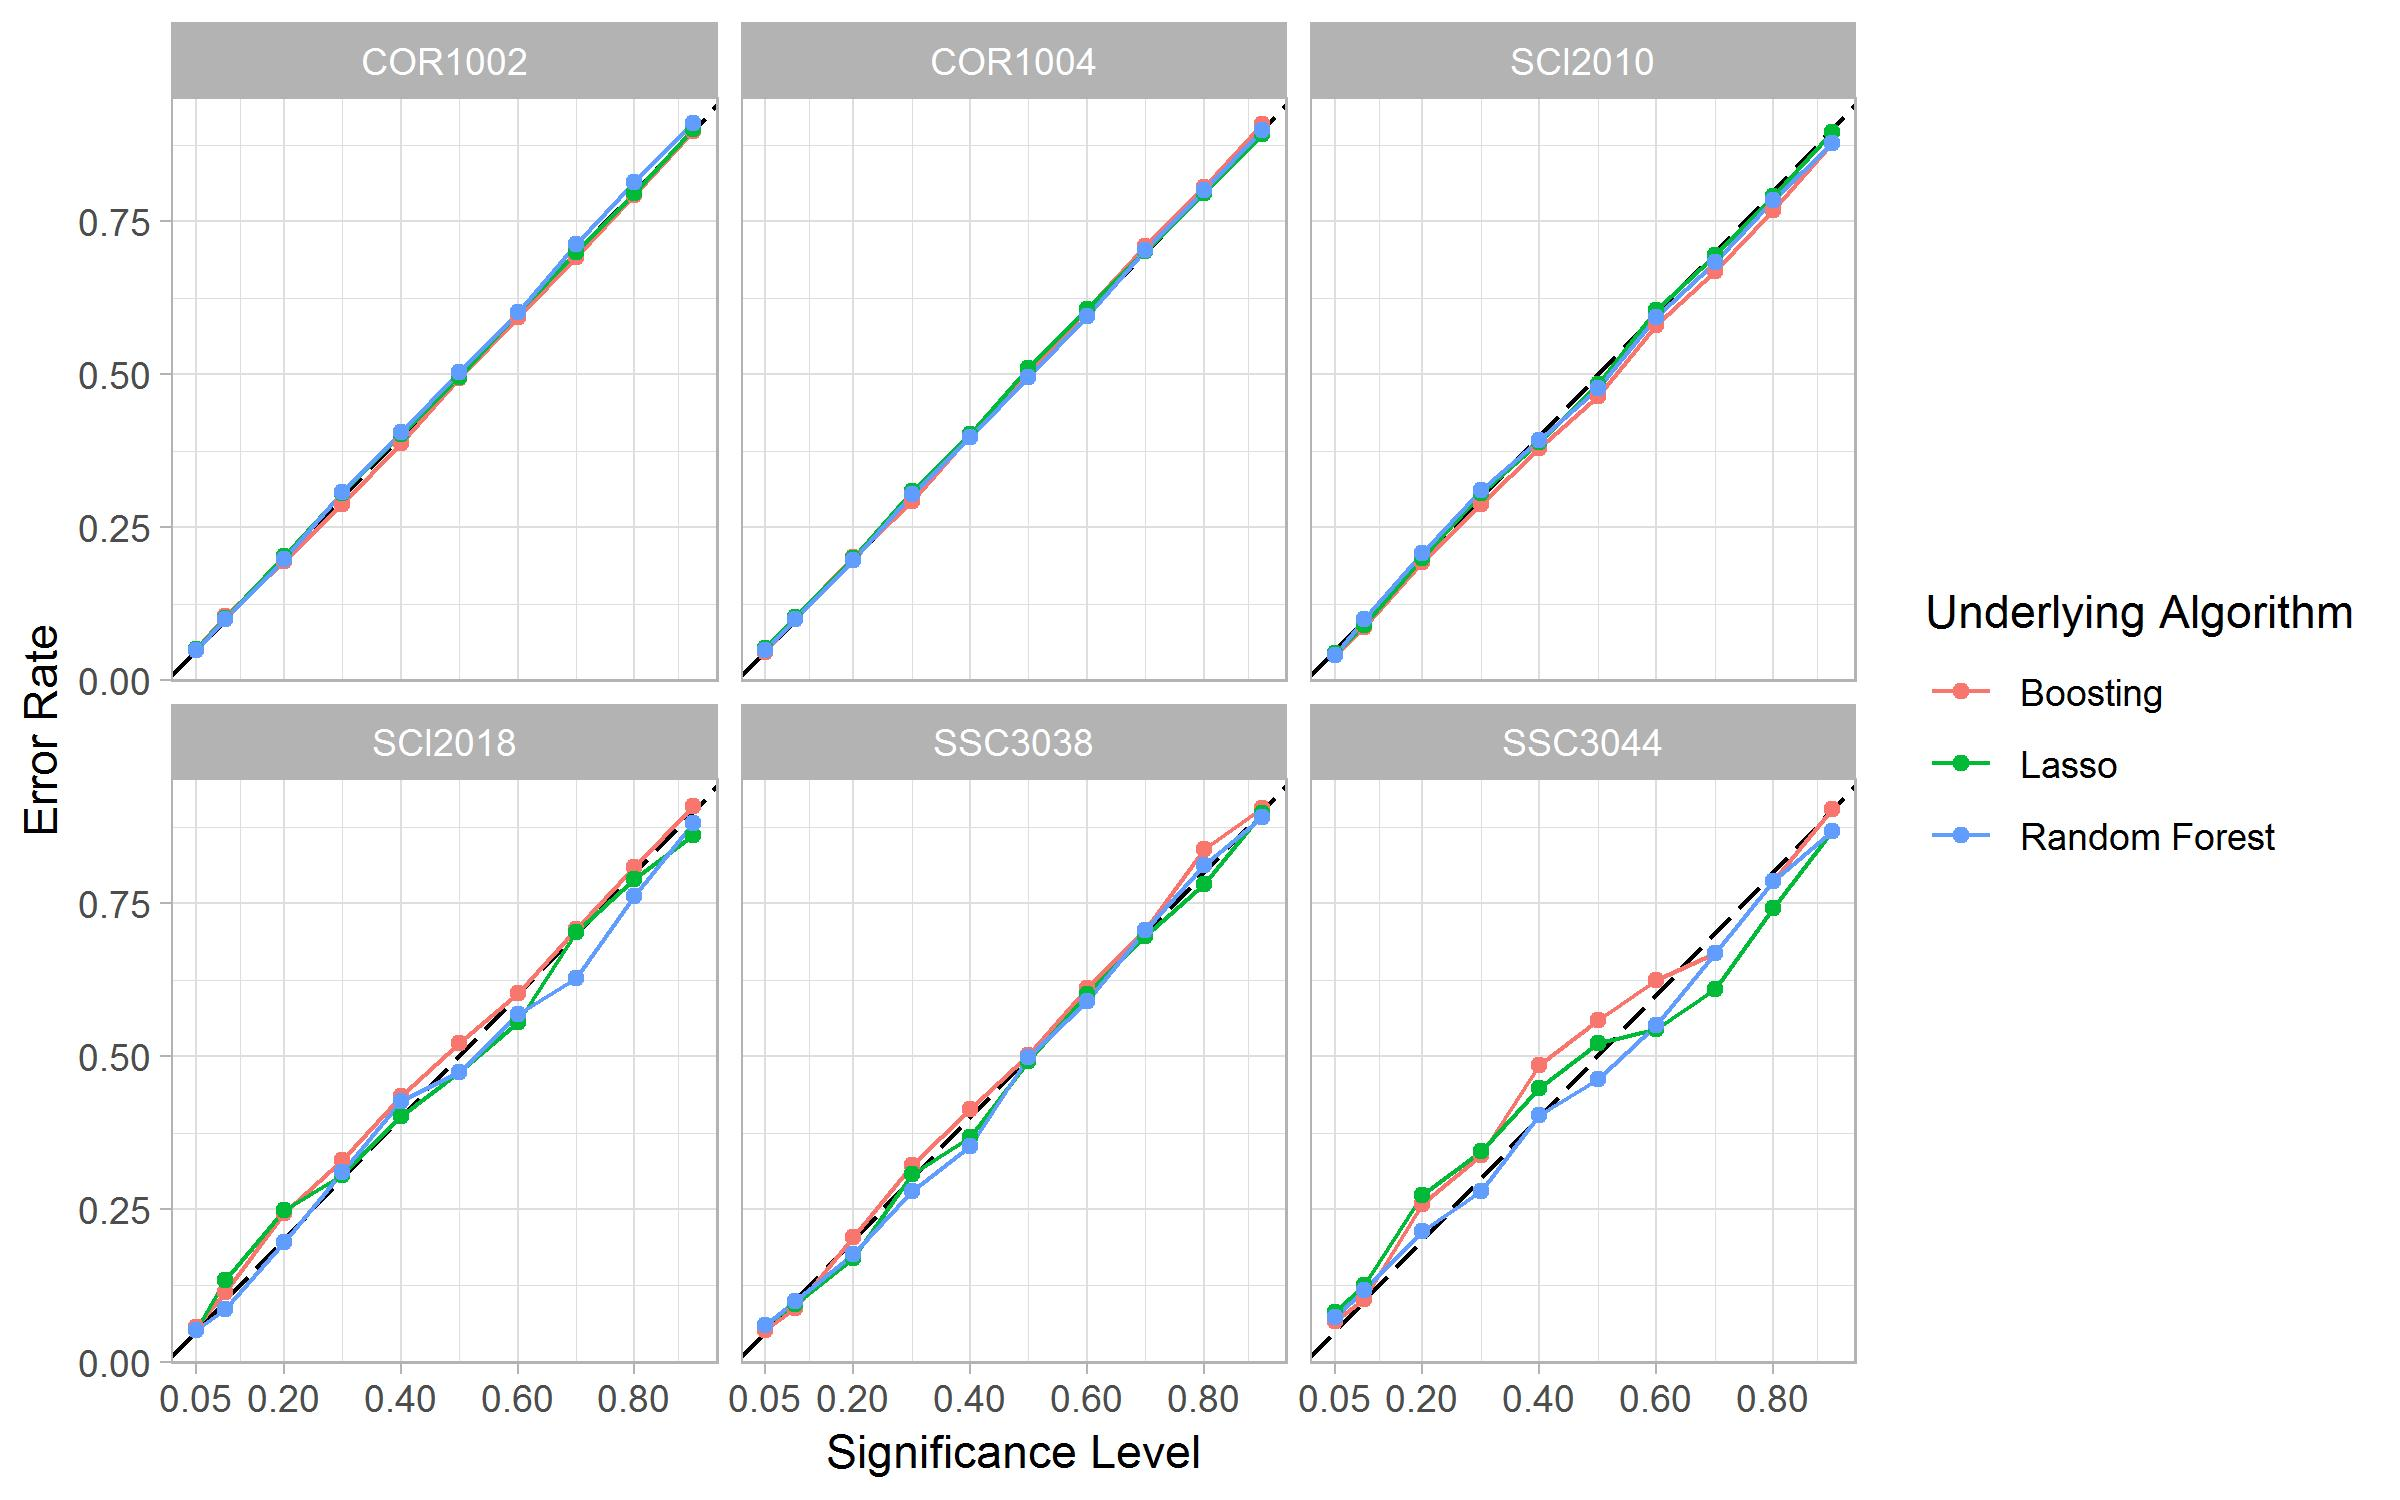
\includegraphics[width=0.8\linewidth]{figures/conformal-error}}
\end{figure}

\begin{figure}[htbp]
	\floatconts
	{fig:conformal-width}
	{\caption{Tightness of prediction interval constructed with the ICM. The dots correspond to the median width and the bars to the 10th and 90th percentiles.}}
	{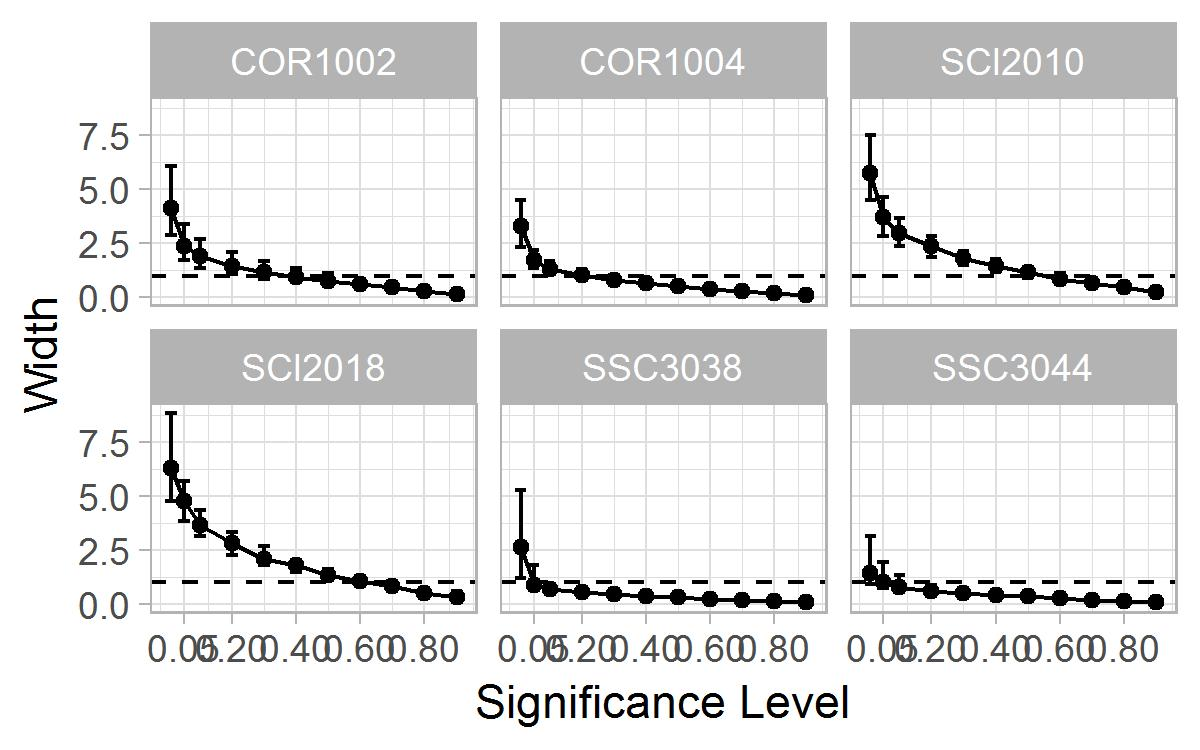
\includegraphics[width=0.8\linewidth]{figures/conformal-width}}
\end{figure}

\section{Conclusion}
\label{sec:conclusion}


In this paper, we complemented LARS's point predictions for course grades with prediction intervals constructed using the conformal prediction framework. We used the ICM with a standardized nonconformity score to construct prediction intervals that are tailored to each student. The results from a selection of 6 courses covering a wide range of sample size and CV mae of the underlying model indicate that the prediction intervals are conservatively valid and that their width seems to be associated with the accuracy of the underlying model. The courses SSC3038 and SSC3044, for example, have the tighter intervals with a median width close to 1 unit at the significance level $0.05$. This result shows that ICM can construct prediciton intervals that are useful for LARS and its pillar 2 for warning issuance.

Yet, courses whose underlying model lacks accuracy end up with prediction intervals that are too wide to be useful. To make the intervals tighter, we will consider two approaches in our future research. First, we will try to improve the performance of the underlying regression model by considering methods that tend to be more accurate than Lasso regression, such as random forests or gradient boosting. Second, we will improve the informational efficiency of the ICM with cross-conformal prediction \citep{Vovk.2015} or its faster version \citep{Beganovic.2018}.

\acks{Our thanks to the University College Maastricht, Maastricht University, the Institute of Data Science, the Department of Data Science and Knowledge Engineering, and in particular to Peter Vermeer for initiating the project and enabling collaboration with the University College Maastricht.}

\bibliography{bibliography}

\end{document}